\RequirePackage[hyphens]{url}
\documentclass[sigconf]{acmart}

\usepackage{hyperref}

%\usepackage{endfloat}
%\renewcommand{\efloatseparator}{\mbox{}} % no new page between figures

\usepackage{booktabs} % For formal tables

\settopmatter{printacmref=false} % Removes citation information below abstract
\renewcommand\footnotetextcopyrightpermission[1]{} % removes footnote with conference information in first column
\pagestyle{plain} % removes running headers


\begin{document}
\title{Big Data = Big Bias? An Analysis of Google Search Suggestions}

\author{Gabriel Jones}
\affiliation{%
  \institution{Indiana University Bloomington}
  \city{Bloomington} 
  \state{Indiana} 
  \country{USA}
}
\email{gabejone@indiana.edu}

\author{Mathew Millard}
\affiliation{%
  \institution{Indiana University Bloomington}
  \city{Bloomington} 
  \state{Indiana} 
  \country{USA}
}
\email{mdmillar@indiana.edu}


\begin{abstract}
While Big Data can make the world a better place, blind optimism in its infallibility can cause irreversible damage to society if left unchecked. With the mission of ensuring accountability, we debunk the fallacious narratives people tend to tell about Big Data, offering a more realistic discussion of its merits and its limitations. We then explore how analytical or algorithmic bias and sampling bias, two problems that statisticians have faced since long before the onset of Big Data, present pitfalls for deriving knowledge from data. We examine how the ethical implications of these pitfalls can cause serious damage in society. We determine that effective, credible, and ethically sound Big Data analysis must obey the principles of transparency, clear and appropriate objective definition, and self-correcting feedback mechanisms. We examine case studies where academicians and businesses have tested algorithms to study how well they exhibit these principles. We then implement our own test to check for potential algorithmic bias in Google. Based on evidence that certain individuals have been corrupted in part by Google searches allegedly bias against racial minorities, we hypothesize that Google's algorithms systematically exhibit biases against minority groups. We test this hypothesis by examining how Google search suggestions associate certain negative words with names that typically belong to minority groups. We conclude that while our study alone cannot prove or disprove our argument, the evidence in our analysis contradicts our hypotheses, thus suggesting that no systematic bias is exhibited. We discuss end by discussing what the results could mean for future studies of potential algorithmic bias in Google.
\end{abstract}

\keywords{i523, hid104, hid216, Big Data, Ethics, Algorithmic Bias, Sample Bias}

\maketitle

\section{Introduction: Fallacious Narratives about Big Data}

Since its origins, Big Data has promised to revolutionize the world. Scholars have wisely noted that it represents a paradigmatic shift from conventional norms of data, but the public has latched onto provocative yet unrealistic narratives that deify Big Data as omniscient, infallible, and impervious to bias. Confiding in such narratives diminishes the integrity of credible science and poses serious ethical challenges, but these challenges are more likely overlooked because the problematic narratives seem to reject the need for ethical discussion. 

In 2008, {\em Wired.com's} Chris Anderson wrote an article that captures the general optimism with which people conceptualize Big Data. The article, with its self-explanatory title ``The End of Theory: The Data Deluge Makes the Scientific Method Obsolete'', argues that Big Data provides such a complete, infallible view into reality that we no longer need conventional methods of scientific inquiry but need only to look at what the data tell us. According to Anderson, ``With enough data, the numbers speak for themselves''\cite{Anderson2008}. This fervorous optimism was further extended in a 2013 book by Mayer-Schonberger and Cukier titled {\em Big Data} where authors assert that Big Data is synonymous with all data. In the past, researchers could only look at samples of data with limited scope, but Big Data, the authors claim, represents not a sample but a complete set\cite{Lagoze2014}. A dataset of Twitter posts is viewed as synonymous with a complete, unbiased set of all of society's thoughts. By analyzing such a dataset, they conclude that they can confidently answer any question about how all of society thinks and behaves\cite{Harford2014}.

Cheerleaders for Big Data, such as Anderson, Mayer-Schonberger, and Cukier to make five exciting but yet flatly incorrect claims: that bigger is always better; that data analysis produces indisputably accurate results; that every data point can be studied, eliminating the need for archaic statistical sampling techniques; that studying causation is no longer needed since correlational patterns tell us all we need to know; and that scientific and statistical models are obsolete, since Big Data is itself sufficient. They have tended to extrapolate from the early success of the Google Flu Trends which at the time successfully embodied such grandiose, idealistic views. The Google Flu Trends project employed a theory-free set of algorithms that studied search engine results to predict flu outbreaks faster and more accurately than the Center for Disease Control. Allowing the numbers to ``speak for themselves'', Google determined that the number of searches about the Flu were correlated with flu outbreaks, so they concluded that more searches could accurately predict a greater spread\cite{Harford2014}. 

At first it worked brilliantly. But in February 2013, just a month before the {\em n = all} proposition was published in {\em Big Data}, it made headlines for failing miserably, overestimating actual trends in 2013 by over 140 percent, leading Google to humbly terminate the program. The overconfidence of such an enormous dataset, viewed as a complete representation of reality free of gaps or inconsistencies, blinded them to its inherent flaws. For one, searches involving the term {\em influenza} are hardly an unbiased determinant of flu prevalence. They committed a classic statistical mistake by failing to consider confounding variables: the other reasons why people might search for the word {\em influenza}. Rather than adapting their model to fit changing patterns in the data, they assumed that the numbers could speak for themselves\cite{Harford2014}. 

But blind proponents of Big Data bury the Google Flu Trends fiasco as just one not particularly convincing counterexample, giving superficial explanations that do not challenge Big Data's position as an infallible deity. In reality, such failure is the rule rather than the exception. Even Gartner, a company publicly known for pushing the importance of Big Data, estimated that 60 percent of Big Data projects would fail\cite{Gartner2015}. But it's not just a matter of occasional success or failure; many people in all disciplines misunderstand the nature of Big Data and therefore have unrealistic expectations. The narrative of the Target coupon case shows that society still regards the potential of Big Data as omniscient even if its execution is occasionally flawed. The story is narrated somewhat as follows.

In 2012, Target had collected enough purchasing data about pregnant women that they determined a particular high school girl was pregnant. When coupons for baby care items mixed in with general coupons started showing up in the mail, the father angrily visited the store manager to complain, suggesting that the store was encouraging teen pregnancy. The manager understood his frustration and called twice to apologize, but on the second call, the father's mood was different. The father offered his own apology because Target was right. His daughter was pregnant, and Target's Big Data analytics managed to discover this before him\cite{Duhigg2012}.

While such a rose-colored narration fits well within the aforementioned grandiose conceptions of Big Data, a closer look shows that this successful case is overblown. While the anecdote seems to prove that Target's algorithms are infallibly accurate -- that everyone receiving baby care coupons is pregnant -- this is very unlikely. While the popular account suggests that Target mixes in coupons targeted towards pregnant women with other coupons to avoid spooking such women about their algorithmic accuracy, a much more credible explanation is that many women see mixed advertisements precisely because Target is unsure which ones actually are pregnant\cite{Harford2014}. Even women who Target does suspect are pregnant have shopping interests outside of baby care items. While the algorithms help not to waste money by sending the coupons to, say, a single male adult living alone, they hardly indicate any reliable accuracy of pregnancy prediction. Of course, this is an empirical question that could be answered by researching how often pregnancy-targeted ads are sent to pregnant women versus those who aren't. But without having a methodologically sound study prove consistent accuracy, it's unwise to extrapolate from the anecdote and assume that Big Data done right is omniscient.

Critiquing the dominant reading of the Target case is not meant to suggest that Big Data has no value. Afterall, Target likely improved the efficiency of targeted advertising through Big Data by more accurately segmenting those who {\em might} be pregnant. But the important thing to keep in mind is that ultimately, models of the world and the data that feed them are imperfect. Models reflect the biases of those who create them, and data reflect biases inherent in sampling methods, time periods, and society in general. Cathy O'Neal, a former professor and Wall Street algorithm specialist with a mathematics degree from Harvard, observes that any model of the world ``begins with a hunch, an instinct about a deeper logic beneath the surface of things''\cite{Wharton2016}. Human potential for bias and faulty assumptions can creep in. Of course, hunches or working thesis provide a necessary part of the scientific method of inquiry. Human intuition can be useful, as long there exist mechanisms by which those hunches can be evaluated and revised when necessary\cite{Wharton2016}.

Perhaps the most common example of successfully wielding insightful models is depicted by the movie {\em Moneyball}, based on a true story. Oakland A's General Manager Billy Beane hypothesized that conventional performance metrics were overrated whereas more obscure measures better predicted overall success. He worked with statistician Bill James to create models that helped Beane decide which players to acquire and which to let go. The once obscure method has become a staple of baseball analytics. According to O'Neal, the model works for three main reasons: it allows for transparent analysis; its objectives are clear and appropriately quantifiable; and it includes a self-correcting feedback mechanism of new inputs and outputs, allowing it to be honed and refined. Models go wrong when they lack these three healthy attributes: ``the calculations are opaque; the objectives attempt to quantify that which perhaps should not be; and feedback loops, far from being self-correcting, serve only to reinforce faulty assumptions''\cite{Wharton2016}.

But models are only one factor in determining the efficacy of Big Data analysis. Since the very nature of data analysis is to extrapolate from limited samples, not only must researchers realize that models include human bias, but data itself is imperfect. It's true that data never lie. But it's false to assume they tell the truth. Data by themselves don't say anything; they simply are\cite{Crawford2013}. No matter how large and complex a dataset, it is always up to researchers to interpret the data to make meaningful claims. This is the essence of the scientific method that some want to reject.

\section{Algorithmic and Sample Bias: The Threats that Never Disappeared}

Humans, as imperfect beings, should never assume that our creations are without flaw and bias. In many ways, mistakes and flawed thinking can trickle into the processes we come up with. This is the idea behind the fallibility of models created by humans with respect to algorithms used for handling Big Data. Some algorithms come with biases based on narrow thinking with a broad scope to cover. Other biases come from the assumption that the Big Data set being used is representative of the population when it really isn't. In any scenario, the creator is prone to introducing bias into any given algorithm, which can make it difficult to trust the results that the algorithm produces. With this in mind and considering the importance of specific findings, there is a lot at stake here. In some cases, lives can be changed for better or worse.

Sometimes algorithms, as models laden with the biases of their creators, can unintentionally manipulate readings of data in ways that reinforce false positives. But not all algorithms are wrong. In fact, machine learning shows us that often a well-written algorithm fed with good data can outperform human knowledge on everything from chess to medical diagnosis. But there's a problem with Big Data; it's inherently messy, complex, and distorted. Contrary to popular opinion that views it as a perfect representation of reality -- recall the {\em n = all} proposition -- Big Data is a black box where typical issues with data quality hide themselves rather than disappearing. No matter how large or complex the dataset, the old adage still remains true: garbage in, garbage out. 

{\em The Literary Digest} experienced the concept of garbage in, garbage out firsthand during the 1936 US presidential election, which pitted the Republican Alfred Landon against the wildly popular democrat Franklin D. Roosevelt. Roosevelt was particularly popular among the working class, the US majority, whereas Landon resonated well with the upper middle class and elites\cite{Harford2014}. {\em The Literary Digest} Tried to predict the outcome of the election by sending out surveys to its own subscribers and by looking people up in phone and automobile registries. During the great depression, the people that owned phones, cars, and subscribed to the  {\em The Literary Digest} tended to be more affluent and republican. After sending out 10 million ballots and receiving back nearly a fifth of them, they predicted that Alfred Landon would win with an astonishing 57 percent of the popular vote. They could not have been more wrong. Landon earned less than 40 percent of the popular vote, losing by a landslide\cite{Crossen2006}. This case has become the archetype example that data from a bias sample will lead to bias results. Increasing the volume of bad data only succeeds in producing a very precise incorrect conclusion, creating a false sense of confidence in something inherently wrong.

Although the {\em The Literary Digest} used lots of data, by definition their sample did not involve Big Data\cite{Lagoze2014}. But if we reject the {\em n = all} proposition, we can see that Big Data is still a sample and is therefore potentially vulnerable to sample bias. But while any statistically literate person can understand what went wrong with {\em The Literary Digest}, sample bias with Big Data is much more complicated and difficult to identify. For many people, random samples of social media data appear impervious to sample bias. Researchers conducting Twitter sentiment analyses often claim objectivity in representing the real world accurately, concluding that patterns observed in these vast, complex webs occur the same way offline. Despite the conflation of people and Twitter users, the two are not synonymous. Twitter users are by no means representative of the population. A Pew Research project in 2013 found that US-based Twitter users ``were disproportionately young, urban or suburban, and black''\cite{Boyd-Crawford2011}. To complicate things further, we cannot assume that Twitter data accurately represent how users behave because users and accounts are not a one-to-one relationship. Some accounts have multiple users, and some users own multiple accounts. Some accounts are just bots that automatically produce content, and some accounts are created and forgotten, going years without use. Furthermore, among active accounts, data are skewed by how some accounts dominate the discourse. Whereas some users post multiple times per day, others use the site only to view content. In fact, 40 percent of active users view content without making contributions, according to 2011 data from Twitter Inc\cite{Boyd-Crawford2011}. The notions of what it means to be active, to participate, and to be a user require critical examination that's almost universally lacking.

The aforementioned examples highlight problems with available Twitter data, but there's also a problem with the integrity of available data. Twitter only makes a fraction of its data publicly available through its APIs. The supposed firehose of data theoretically contains all public tweets but explicitly excludes data that a user chooses to make private. Furthermore, theory does not match reality as the firehose lacks some publicly available tweets. Very few researchers get adequately full access. Research by Microsoft's Danah Boyd and Kate Crawford found that rather than a firehose, most have access to a ``gardenhose (roughly 10 percent of public tweets), a spritzer (roughly 1 percent of public tweets),'' or just select access through whitelist accounts\cite{Boyd-Crawford2011}. Not only are protected data excluded, but data samples are not always randomized. So, a more reasonable description of Twitter data would say it takes a skewed sample of the real world population, further skewed by how users and bots create or do not create content, and then it limits the scope of the skewed data in an often opaque, arbitrary manner\cite{Boyd-Crawford2011}. Is this data useful? Without a doubt. Is the data so perfect and infallible that we need not concern ourselves with basic principles of statistical and scientific credibility because ``the numbers speak for themselves''\cite{Anderson2008}? Not even close.

If an algorithm could analyze a large, random sample of every word ever thought, spoken, or written by every human throughout their entire life, we could confidently believe that {\em n = all} and make a sentiment analysis that accurately captures how people feel about a certain topic without regard for methods of scientific inquiry; the numbers would ``speak for themselves''\cite{Anderson2008}. But we do not, and probably never will, have that kind of data. Twitter or other social media platforms are no substitute. While understanding the fallibility of Big Data is perhaps not as clear and straightforward as the {\em Literary Digest} case, society must be responsible by diligently scrutinizing data. To paraphrase loosely from world-renowned consultant Meta S. Brown, the biggest problem with data analysis will always be people failing to admit that data imperfections exist, failing to look for them, and refusing to do anything constructive about the ethical implications of these imperfections\cite{Brown2017}.

\section{Ethical Implications of Algorithmic and Sample Bias}

As we've seen, the massive failure of the Google Flu Trends caused embarrassment and wasted Google's money. But the consequences they faced are relatively trivial, and given the company's history of learning from the past, they are probably a better company because of the failure. But when Big Data goes awry, the consequences are not always so trivial and localized. Big Data used unwisely has very serious, irreversible impacts upon society. Pervasive overconfidence can make it harder to acknowledge and confront such impacts until too late. 

Society's current failure to address these issues is the topic of Cathy O'Neal's book {\em Weapons of Math Destruction: How Big Data Increases Inequality and Threatens Democracy}. She argues that these WMDs, referring to Big Data algorithms, have good intentions but often reinforce harmful stereotypes, especially of minorities and the poor, and become opaque models wielding arbitrary punishments. Through her work in the private sector, she has experienced numerous Big Data horror stories, and the book discusses several different failings of Big Data in various contexts.

One common issue associated with Big Data is the notion of self-fulfilling prophecy: the idea that expectations change reality to make it reflect the expectations. If police suspect African Americans to be more likely to commit crimes, they may patrol black neighborhoods more often and proactively hunt criminal activity. Increasing patrols increases the number of arrests, which provides justification to further increase patrols, causing more arrests, and so on. The prophecy that African Americans are more likely to commit crimes becomes adequately reinforced with their higher incarceration rates. But higher likelihood of arrest is not the same thing as being more likely to commit crimes\cite{Liu2017}.

It should be easy to see how the example of arrest rates is problematic, but somehow incorporating Big Data tends to make people fail to recognize the possibility of self-fulfilling prophecy. In fact, numerous police departments use algorithms that do just this, inadvertently instructing their officers to focus on areas with high concentrations of blacks. Crime prediction software that attempts to adjust police deployments according to anticipated patterns fail when they confuse more data with better data. Even though they attempt to prioritize violent and serious crime, data generated by relatively insignificant petty crimes, which occur far more often in poor and predominantly minority communities, can overwhelm the system, making it prejudice. Once the petty crime data enters a predictive model, more police deploy into those neighborhoods, and they are more likely to arrest people by their sheer presence and by the perceived threat that those people pose. The increased arrests justify the deployments in the first place\cite{Wharton2016}. 

But the danger does not end there. Once people are arrested by these inherently discriminatory processes, Big Data can work to keep them in prison for longer. This is usually not by intention but by flaws in design. Recognizing how unconscious bias can affect sentencing decisions, courts in 24 US states have started to use computerized models to help assess the risk of recidivism, the likelihood of repeat offense. The models attempt to use Big Data to avoid a common, serious problem with human reasoning, and they certainly show some promise in this regard. But over reliance on the models can prove even worse than trusting potentially bias judges. ``By attempting to quantify and nail down with precision what are at root messy human realities'', the recidivism models shroud sentencing bias in a veil of unwarranted confidence and precise accuracy that disadvantages minorities by subjecting them to harsher prison sentences\cite{Wharton2016}.

How does one quantify something as complex as the risk of recidivism? One popular model uses a lengthy questionnaire that attempts to pinpoint factors related to this risk. The questionnaire inquires about things such as previous police incidents. Given how much more often young black males get stopped by the police, partly because of the aforementioned self-fulfilling prophecy, such questions easily become a proxy for race, despite intentions to reduce this very prejudice. Other questions, such as whether or not the respondent's relatives or friends have criminal records, would be flagrant violations of court procedures and surely elicit objections from a defense attorneys if raised during a trial. But the opacity ``of these complicated risk models shields them from proper scrutiny''\cite{Wharton2016}. Discriminatory police strategies feed into the recidivism models used to call for harsher sentencing, creating ``a destructive and pernicious feedback loop''\cite{Wharton2016}.

It is no secret that racial tension has become a dominant source of discussion when it comes to the American justice system. However, this issue is compounded with bias produced within the data itself as well. When there is a bias in how arrests are made based on the color of someone's skin, this bias feeds into an algorithm which opens up for more bias down the road. As more people of a given color are arrested and given harsher sentences, this data builds up in the system. The root of the cause may be human bias, but there is definitely a healthy amount of algorithmic bias that compounds and builds on the issue as most algorithms lack the ability to look beyond the face value of the data provided\cite{Eckhouse2017}.

Big Data is, of course, not only used in attempts to more effectively dole out punishments. Facing international competition, Corporate America has latched onto its potential for increasing profits through more effective marketing, financial trading, and personnel decisions. With the prevalence of the internet, social media, and information literacy, Big Data presents an enormous opportunity for market personalizing. Rather than targeting advertisement campaigns on broad, general audiences, Big Data can segment down to the individual level, targeting people based on their own personal data and patterns of behavior. However, this type of marketing is still a very inexact science and raises tricky ethical issues, including gender bias. Like racial bias, gender bias comes about in scenarios where profiling usually happens. For instance, advertising on the internet aims to reach its intended audience in order for businesses to sell products and make profits. Big Data and the statistical analysis involved might suggest that a certain gender has specific tendencies or lean on embedded societal stereotypes which cause some serious bias in an algorithm. One example might be a job opportunity being advertised. In this case, we want to say that either gender should be shown the advertisement a near equal amount, but we know from experience and outrage that this is not the case. It is almost staggering how it would favor the male population at times, especially when dealing with high paying jobs. Here, we also have a combination of Big Data and algorithmic bias working hand in hand to create biased results that ultimately lead to insult and faulty representation\cite{Brown2017}.

Beyond marketing, Big Data has found particular popularity among Wall Street investment firms, and for good reason. The ability to incorporate Big Data into decision making has tremendous potential for profitability. But the subprime mortgage crisis demonstrated how this can also have tremendous destructive potential. Financial models exhibited a particular bias, reinforcing the idea that what has worked in the past or what works currently will continue working indefinitely. But the sophisticated mathematical models lacked self-correcting feedback that could indicate inherent flaws. Since the models were driven by the market, if they led to maximum profits, they were considered infallible. Otherwise, why would the omniscient invisible hand of the market reward it? In hindsight we all recognize that betting on the subprime mortgage bubble was a losing proposition, yet the myopic reliance on the market proved disastrous in 2008. During the financial crisis, the algorithms used to assess securities risk became smoke screens. Their complex, mathematically intimidating design ``camouflaged the true level of risk''\cite{Wharton2016}. The opaque models also lacked a healthy feedback mechanism that could have identified the problem\cite{Wharton2016}. The severity of the 2008 recession shows that companies are not only accountable for their own success and failure. Their misuse of Big Data had broad sweeping effects across the entire economy.

Perhaps it is reasonable to understand why companies might get carried away in a practice that, at least on the surface level, does not appear to affect humans directly. A trader working on the top floor of a Wall Street skyscraper might not see how the work of his mathematicians might hurt or harm average people. But Big Data also plays a role in ways that very clearly affect individuals, especially with the increasing popularity of integrating technology into personnel decisions. Since personnel decisions directly impact company performance, workforce management has become popular, particularly programs that promise to eliminate the guesswork from hiring by screening potential employees \cite{Wharton2016}. Many of these programs use personality tests to try and automate the hiring process; 60 percent to 70 percent of prospective employers, according to Deloitte Consulting.

Despite the optimism, such tests face the same problem as the recidivism surveys: they try unsuccessfully to quantify and precisely measure ``what are at root messy human realities''\cite{Wharton2016} The high use of personality tests goes against research that consistently shows them to be poor predictors of future job performance. They don't provide this goal but rather an illusion of objectivity and simplicity. They generate raw data that get plugged into efficient algorithms and give clear answers, as opposed to the time consuming and obviously subjective process of human interviewing. Not only does this illusion cooly deceive companies, it leaves prospective employees disgruntled and confused by results from a opaque systems. Rejected employees don't know if they've been flagged or what caused them to be. The personality tests also lack important feedback mechanisms. There is no way to identify inherent errors in the model and use those mistakes to refine the system\cite{Wharton2016}. Far too often, personality tests fail both the companies that use them and the prospective employees that get arbitrarily denied a chance.

In each of these cases, the story repeats itself where ethical issues that are normally fairly obvious become invisible when Big Data enters the picture. The argument is not that we should reject the positive potential of a reality that will only grow stronger with time. Rather, we should remain cognizant that a failure to adhere to basic principles of scientific credibility and ethical reasoning can affect people in unseen but deadly ways.


\section{Potential Algorithmic Bias in Google: The Dylann Roof Case}

Sometimes, algorithmic bias can morph and distort opinions in ways that almost seem like indoctrination in nature. In some cases, it can seem like this bias can be the root of a terrible downward spiral into blatant racism, but when do we justifiably point blame at the machine rather than a person's inner desires? In today's society, it can be tempting to take the easy way out of tough situations and place the blame anywhere else that might make sense as long as it provides some kind of vindication. That being said, we do live in a generation that is gradually becoming more influenced by the internet and technology in general as the years fly by. With that in mind, it is reasonable to see where a flaw or bias in an algorithm can have a monumental impact in a negative way on some people. Unfortunately, there have been cases where people are significantly effected by these algorithmic biases in ways that trigger a violent disposition towards another group or race.

In 2015, a man named Dylann Roof shot and killed nine people at a church in Charleston, South Carolina. The interesting details hanging around this massacre to make it stand out were the people he shot and the line of reasoning he used to explain how he was eventually led to commit such an act. The attack was done on what was reported to be a predominantly black church which led people to label the offense as a hate crime. However, Roof's explanation on what might have led him to that point is what makes this story stand out from other hate crimes. In an article that the National public radio published titled ``What Happened When Dylann Roof Asked Google For Information About Race?'' it was reported that Roof's defense had made a case that there was more to the act than just simple racism and white supremacy\cite{Hersher2017}. The argument that the internet had a direct influence on what Roof believed and that he was acting on the information he was being fed through other sources was being made. Roof elaborated on the subject and explained that it had all begun with the growing popularity of the Trayvon Martin case. Trayvon Martin was an unarmed black teenager who was shot and killed in 2012. After researching the details of the case and coming to his own conclusions he states in a quote in the article ``this prompted me to type in the words 'black on White crime' into Google, and I have never been the same since that day''\cite{Hersher2017}. The article continues to dive deeper into what Roof might have encountered. Anyone who has encountered a search engine in general has been faced with the auto complete feature that provides calculated, popular options to give the user some direction. In this case, the potential algorithmic bias surrounding the racial tensions might have led Roof down the path of searching for examples of crime committed by people of color on white people. The National Public Radio itself reported that they tested out Google's search engine by typing out the beginning of the phrase Roof mentioned and they were prompted with the auto complete option of the exact phrase before they could even type in the word white\cite{Hersher2017}. Even today, you can perform the same experiment and come up with the same results.

Unfortunately, the main factor in driving this algorithmic bias is popularity and relevance which are hard variables that are difficult to counter and account for in most cases. This means the objective of removing the type of algorithmic bias that Dylann Roof encountered would be difficult and require a major change in how search suggestions and results are calculated. However, this needs to be discussed and changes need to be made or more people will continue to be influenced negatively by algorithmic bias which would put more lives at risk down the road. After all, Roof was only seventeen when he began down the line of thinking that led him to commit those murders. There are numerous children and young adults that have unlimited access to the internet and are wide open to the same influence. So, preventative measures need to be taken in order to assure that we do not see similar stories surface. In order to get that done, there has to be some kind of analysis of bias within specific algorithms to understand them and create ways to account for this bias. If unchecked, not much can be done, but the knowledge from understanding the potential bias in these algorithms could prove invaluable.

\section{Case Studies in Checking for Algorithmic Bias}

Before we can test for algorithmic bias, we have to have a grasp or understanding on how typical algorithms implemented in concepts such as prediction work. In many fields where predictive work is being done in research, there is a common use of natural language processing algorithms such as Support Vector Machines, Neural Networks, and Naive Bayes. Each algorithm uses a specific type of processing that makes it stand out from the others, but the different aspects to each come with advantages and drawbacks that make each one valuable in certain circumstances. However, it is the internal structure of what makes up the algorithm that allows for bias to get in.

\subsection{Support Vector Machines}

A Support Vector Machine is a supervised learning model that is known for the analysis of data for classification and regression. This algorithm is much better at classifying problems than normal logistical regression, and it always converges to a global minima when classifying data. However, this algorithm can be complex especially when the data isn't linearly separable. In the case that the data set being used is non-separable, the data can be transformed using a kernel function, such as a log function in some cases, in order for the algorithm to fit the data and classify correctly. The main bias that we can see from this algorithm is in the case of it classifying data to the point where patterns form based on things like popularity and relevance which could lead to something similar to what we discussed in the case involving Dylann Roof. Since Support Vector Machines are supervised learning models, any bias can be accounted for in the manual make up of the model because it does need some direction. In that case, bias might come in the form of human error though.

\subsection{Neural Networks}

Neural Networks are algorithmic models in which weighted inputs are fed into a function to compute an output. In a predictive setting, Neural Networks are fairly flexible in structure which allows it to be applied in many scenarios. In this type of model, we can expect to utilize logic gates in order to understand how certain scenarios must be weighted to account for a specific outcome or result that we want. If an outcome relying on three variables hinges on a specific variable being untrue and requires at least one of the other variables to be true, we would assign a higher weight to the first variable than the other two because that one variable to ruin the outcome. We can see how this type of modeling can be used to model complex predictive problems and could possibly be used in a search engine if desired. Based on input strings that make up common and popular words and phrases, we could make an auto complete function using neural networks to put weights on certain inputs to predict the possible resulting desired search for the user. Unfortunately, placing weight on certain inputs and pieces of the function can inherit some bias along with it. Even if those weights aren't manually decided, popularity and relevance can have a large impact on calculation of weights which would still lead to some bias down the road. In the search engine example, this would lead to people being influenced to search something based on the beginning of their search query.

\subsection{Naive Bayes}

The Naive Bayes classifier is a probabilistic model that applies Bayes' Theorem that makes predictions based on a set of training data consisting of predetermined features. However, Naive Bayes places the assumption on the features that each one is independent of the other. Although this stipulation does well enough in real word situations, this assumption can hold it back from working in more complex situations where features are highly dependent on one another. In the world we live in today, we rarely encounter situations in large data sets, especially in Big Data settings, where the features involved are independent. This strong assumption of independence here is where the source of a decent amount of bias could come from when using this algorithm. Because of this, there is a limitation to how well one can make predictions in more complex situations. After all, Naive Bayes is a probabilistic model, but probabilities tend to rely on a multitude of varying factors which may include the influences of other features involved.  With this in mind, we can see how the results may be skewed or flawed, but how exactly does that introduce bias? Other biases can come within and there are undoubtedly some in this algorithm, but another major source of bias can come after the work is done. A critical piece comes from the analytic interpretation of the results. If the probabilities are flawed, then the conclusions made from the results could be flawed as well. In this case, we would call it analytical bias. Even though this type of bias isn't an internal problem of the algorithm, it is a byproduct of it in the end result.

\subsection{How to Check and Account For Algorithmic Bias}

After getting to know what kind of algorithms we are working with and what kind of biases can arise from them, our attention should naturally gravitate towards ways we can check and account for these biases. In some of these algorithms, we can recognize and pinpoint potential biases based on how it acts and the conditions set, but we can also account for a lot of it since Support Vector Machines and Neural Networks are, for the most part, supervised models. This means that some of the biases stem from some programming error which can be accounted for by fixing and tweaking the algorithm. This works for these models because there are main points such as variable weighting and classification in Neural Networks and Support Vector Machines respectively. However, the Naive Bayes classifier is a little more ambiguous. This algorithm struggles with over fitting the data which means that it caters too closely to the data set and prevents it from effectively predicting and adding future data points. In this case, more bias or alteration to the model may be needed to find an equilibrium and allow proper analysis. This requires that less influence be put on handpicking features and allow for a hands off approach. This is often considered soft feature selection in data analytics and is a way of removing the harshness of imposing desired features. With all of this in mind, it is near impossible to completely remove the influence of bias in any given algorithm. There will usually be a flaw somewhere no matter how hard we try to create a perfect model. This is clear when looking back on the Dylann Roof case study about Google algorithmic bias. In the same article, Google indicates that they are aware of biases in their algorithm and that they have worked on eliminating and fixing the issues\cite{Hersher2017}. Even with this awareness and implementation of fixes, we need data and analysis to help us evaluate how well Google improved their algorithm. This was one of our many motivations for testing Google's search suggestions for bias.

\section{Our Case Study: Testing Google for Negative Search Suggestions Bias Against Certain Races}

Based on the observed need for scrutinizing algorithms and inspiration from researchers who have successfully done so, we devised an experiment to test Google's search suggestions for potential bias against names associated with particular races. In the following sections, we discuss our our methodology, our hypotheses our algorithm, and our results.

\subsection{Methodology}

Building off of several researchers and the anecdotal record which have identified cases of bias against certain names, we decided to test for such biases by identifying how negative word associations correlate with searches for particular names. We decided to look for instances of the words associated with {\em arrest, murder, crime, homicide,} and {\em prison}, including the words {\em arrested, arresting, arrests, murderer, murderers, murdering, crimes, criminal, criminals criminality, homicides, homicidal, prisoner,} and {\em prisons}. 

Since we expected these associations to carry bias based on race and ethnicity, we decided to use data that separated names into racial and ethnic categories. To make as objective of an assumption as possible regarding which names were associated with which race, we used data from the 2010 Census that identifies what percentage of people self-identify with which types of names. This allowed us to classify a name as belonging to a certain racial or ethnic group if most people with that name identified under that race. However, one complication of using Census data is that we only had access to surnames. Whereas, based on intuition, a person might be able to distinguish a predominantly Black first name from a predominantly white first name, this is much more difficult for surnames. However, whereas black and white surnames are less distinguishable, Asian and Latino or Hispanic names are much easier to identify because they are usually not based on the English language. For these names, we can be confident that Google recognizes the name and can make associations based partly on these racial and ethnic identities.

Given that the central argument from our qualitative analysis of Big Data suggests that Big Data analysis often has inherent flaws, we determined that avoiding many of the common pitfalls observed with such research should be a top priority. We wanted to study something with which we could be completely confident that the results reflect the true nature of Google's algorithms, whether they support our hypotheses or not. For this reason, despite initially considering it, we decided to avoid studying web page data for such information. Data from web pages would have been problematic because it is difficult to infer the context behind word associations. Simple word counts could create potential false positives. For instance, if a web page from the search {\em Mueller arrest} uses the word {\em arrested} n amount of times, it could be an arrest record report for someone with the last name Mueller, a decidedly negative view, or it could a page talking about the people arrested by order of former FBI director James Mueller. Since our study depends on isolating not only words but negative associations, this lack of context introduces an irreconcilably high level of uncertainty: it would be far too difficult to determine which sites held negative views of the particular name and which ones had positive vies. For this reason, we decided instead to look at search suggestions. Google's algorithms play the central role in search suggestions, and the simplicity of the searches largely eliminates the problem of insufficient context. By just typing in a name and the first few letters of a search term, we can be more confident that whichever suggestions are revealed reflect clearly distinguishable sentiments (negative or positive) regarding the name itself.

\subsection{Hypotheses}

Given the anecdotal evidence and from a history of racial and ethnic bias in the United States, we expected to see a bias toward and ethnic minorities. However, we expected that words associated with criminality would apply much more to Blacks and Latinos than to Asians. Therefore, we hypothesized the following: \\

\vspace{2mm}

{\em H1: Surnames that most often identify Black people will, on average, have more negative word associations than names which most often identify White people.} \\

\vspace{2mm}

{\em H2: Surnames that most often identify Black people will, on average, have more negative word associations than names which most often identify Hispanic or Latino people.} \\
\vspace{2mm}

{\em H3: Surnames that most often identify Hispanic or Latino people will, on average, have more negative word associations than names which most often identify White people.} \\

\vspace{2mm}

{\em H4: Surnames that most often identify Hispanic or Latino people will, on average, have more negative word associations than names which most often identify Asian and Pacific people.} \\

\vspace{2mm}

{\em H5: Surnames that most often identify White people will, on average, have more negative word associations than names which most often identify Asian and Pacific Island people.} \\

\subsection{Algorithm}

The coding for our analysis was conducted with Python 3.5.2. The necessary import modules include: {\em requests, json, csv, urllib.rquest, matplotlib, pandas, scipy, numpy, and timeit}, all of which we installed using {\em pip install}. We gathered the data for our project from the website for the 2010 Census. Their .csv provided us with a list of 162,254 surnames. We read in the file, which is posted in our github account, using csv.DictReader. We isolate the name and race/ethnicity columns. For each name, the race/ethnicity categories include the percentage of people that identify as part of a particular race or ethnicity. Because increasingly obscure names are likely less identifiable, we decided to use only the first 500 names. None of these 500 names were predominantly multiracial or predominantly Native American, so these categories were excluded from our analysis. We created a dictionary with the analyzable categories, {\em pctwhite, pctblack, pctapi, pcthispanic} and sorted the 500 names into the appropriate categories using a series of {\em for loops} that checked for the highest percentage. 

We then move to the main goal of the experiment: capturing Google search suggestions. Using Mozilla Firefox 5.0 as a user agent, we use a url that automatically outputs a two-dimensional list with the search term and ten Google suggestions. We then define a function to modify the url for each search term and for every name. When, for a given name, a search suggestion contains one of the target words described in the methodology section (arrest, crime, homicide, etc.), the function adds a point to the name's value. We run the function five times for each target word, creating five dictionaries that store names as keys and the number of negative word associations as values. We add the five dictionaries to a list that we can iterate through. This section involves a lot of searching, so we use timeit to make sure it runs efficiently. It typically takes about 200 seconds to run with 8 gigabytes of ram and an Intel i7 processor with 500 names, so we estimate that this step would take about 65,000 seconds or over 18 hours to run with the full data.

Now that the search results are appropriately organized by name and by search term, we need to calculate the scores for each race/ethnicity category. We create two dictionaries for each of the four race/ethnicity categories, with search terms as keys and values defaulted to empty lists. For each pairing, one will be later converted to averages and the other will stay as raw data. We then define a function that will appropriately fill the values so that we know how many negative word associations go along with each search term for each race. As inputs, the function takes the name of the racial/ethnic category, the name of the dictionary for that category (from the four we just created), and the list containing the five search term dictionaries we created earlier. The function uses three for loops to iterate through the various dictionaries and lists to match names with their racial categories and add the values to the scores accordingly. We run this function eight times in total for the four pairs of dictionaries.

To calculate the aggregate word associations for each racial category, all we need to do is sum the values of each key for each dictionary. However, to be completely sure that the function for the previous section worked properly, we implement a set of for loops to calculate the aggregates instead of just summing the dictionary values. We create a dictionary with keys set to the racial category and values defaulted to zero and allow the for loops to calculate the proper scores. We also create a dictionary with racial categories as keys and empty lists as values. We append the numerical values for each word association to the empty list. With the data arranged as such in raw form, we are now able to analyze more measures of central tendency, including the median and the 1st and 3rd quarterlies. This data arrangement enables us to create the box plot displayed in the results section. Now, for every pair of category dictionaries, we use one of the dictionaries to calculate averages of the aggregate data so that we know how many negative word associations go along with each name and each search term on average. 

As a final data preparation step, we are now ready to conduct statistical analysis through a separate .csv file. We write out the data name-by-name to a .csv file by using a series of {\em for loops} that arrange the data row-by-row grouped by the race it belongs to. The {\em for loops} arrange everything into a long string with new line characters to separate where each row should be, and then we write it out in one step. From there we read in the new resultsdata.csv file with csv.DictReader and sort the data totals data into numpy arrays by racial/ethnic category. We then conduct two sample t-tests to compare each array to calculate statistical significance. With this step, we now have all the data summarized and organized as needed and can move on to to creating a bar chart, a box plot, and a series of radar charts using matplotlib. Details on how to recreate these visuals are available on the Jupyter notebook on our github project folder.

\subsection{Results}

While we had qualitative data that suggested Google's algorithms could be biased against Black and Hispanic/Latino minorities, the results do not support most of our hypotheses. Regarding H1, while Figure 1 and Figure 2 appear to show that Black surnames do have more negative associations than White surnames, the results were not statistically significant at the .95 confidence level (p \textgreater .85), so we conclude the null hypothesis in this case. This lack of statistical significance is likely due to the very small number of Black surnames (9) compared to White names (361) in the top 500.

\begin{figure}
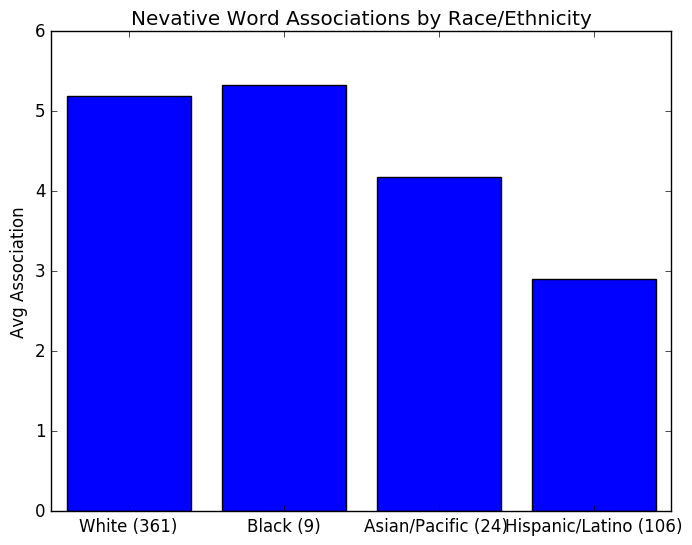
\includegraphics[width=\columnwidth]{images/fig1.png}
\caption{Bar chart comparing average word associations by race.}
\label{Figure 1}
\end{figure}

\begin{figure}
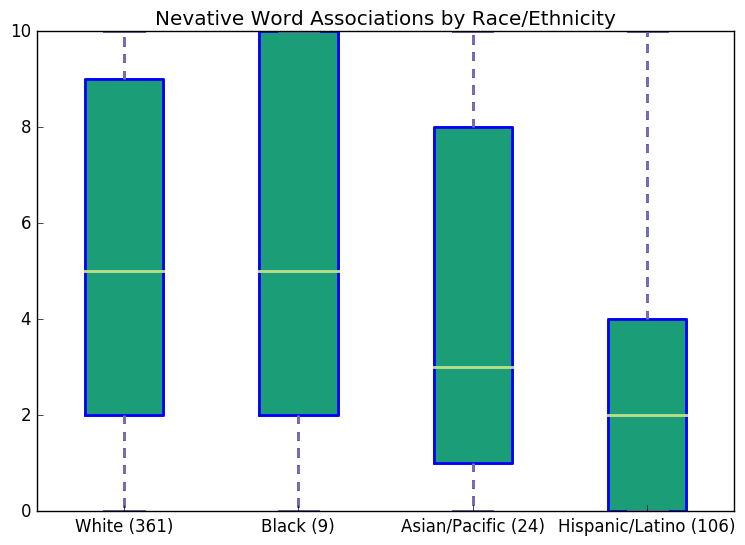
\includegraphics[width=\columnwidth]{images/fig2.png}
\caption{Box plots showing distribution of average word association by race.}
\label{Figure 2}
\end{figure}

Comparing Blacks to Hispanics with H2, however, Figure 1 and Figure 2 do clearly support our conclusion. The difference in means is about 2.4, and this difference is significant at the .95 confidence level (p \textless .002). With a mean of just 2.9, the average negative associations for Hispanic/Latino was actually the lowest in the data set, so H3 was not just nullified, but the exact opposite is true with statistical significance: White names had more associations than Hispanic/Latino names. Hispanic/Latino names also had fewer negative that Asian/Pacific Island names, so we also reject H4. While Asian/Pacific Island names did not have the lowest amount of negative associations, the group did have significantly fewer than both White and Black names, so we can confirm H5. H5 and H2 were the only hypotheses that were supported by the data; H1 was nullified, and for both H2 and H3, the opposite was shown to be true. Given that our hypotheses were not supported, we cannot support our central claim that Google search suggestions would have inherent biases against Black and Hispanics/Latino surnames based on negative word associations dealing with the identified search terms.

Along with our other visualizations, we included a few radar charts showing the distribution of negative search results based on the word we focused on, as seen in figure 3 and figure 4. One with the four races separated into their own chart and the other with all four races overlapping in one radar chart. The idea behind this observation was to get an idea of which words impacted the negative results the most. The charts do not have a significant impact on our original hypotheses, but are there to just give us general insight into the data. However, by observing the charts, we can see that the three most negatively associated search words across all races were crime, arrest, and prison in no particular order across all races.

\begin{figure}
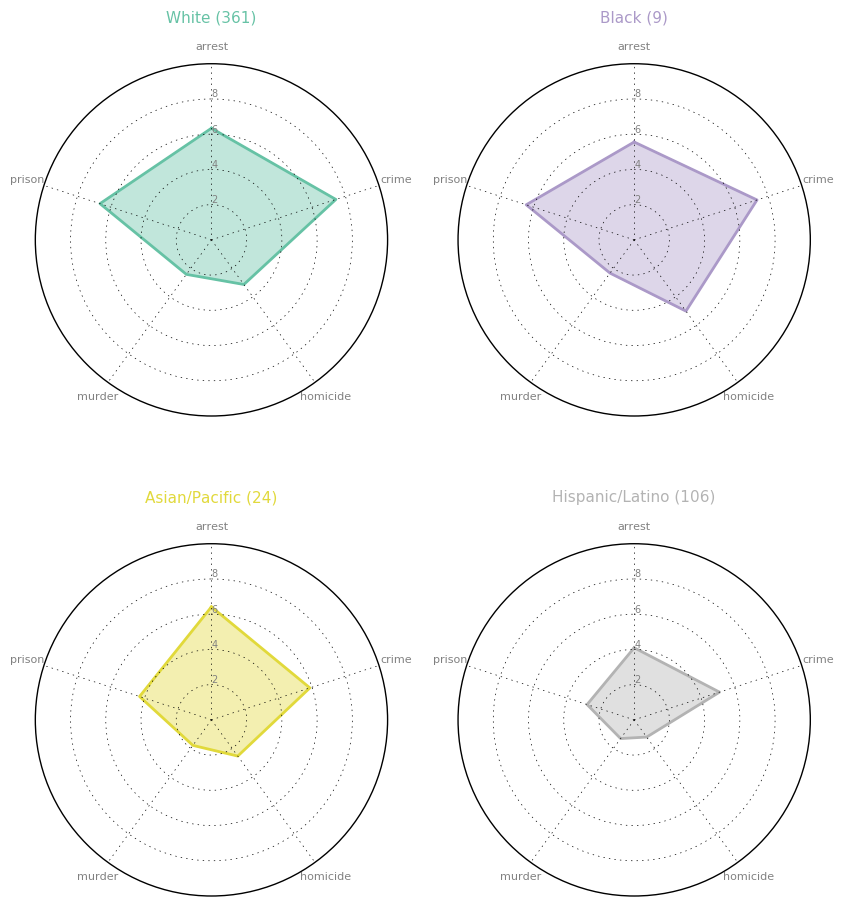
\includegraphics[width=\columnwidth]{images/fig3.png}
\caption{Series of radar charts showing average word association by race and by search term.}
\label{Figure 3}
\end{figure}

\begin{figure}
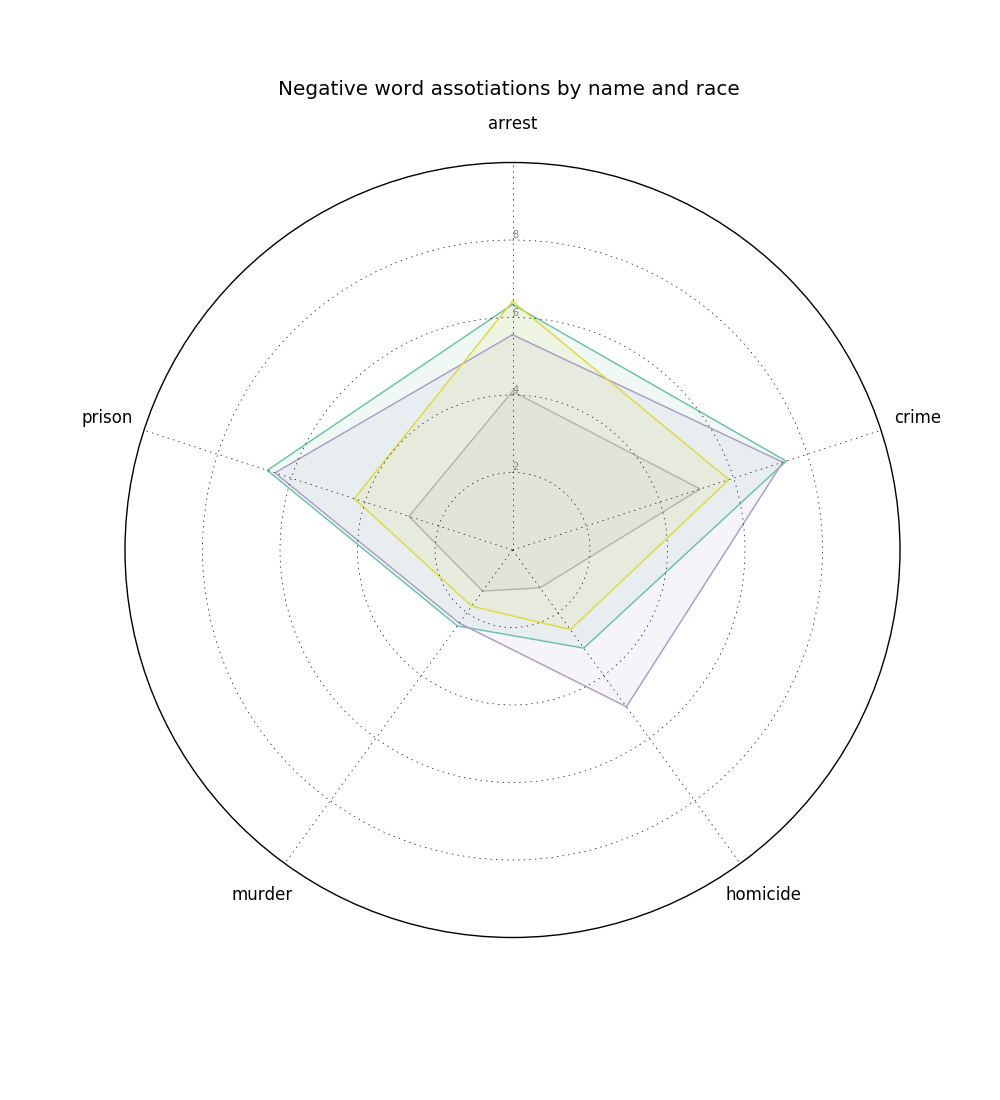
\includegraphics[width=\columnwidth]{images/fig4.png}
\caption{Consolidation of the previous four radar charts into one image that shows how each race compares.}
\label{Figure 4}
\end{figure}

\section{Discussion}

While our results did not support our assumptions, this does not necessarily mean that Google does not exhibit any forms of algorithmic bias. However, it does suggests that, Google is probably quite aware of accusations of bias, like the ones following the Dylan Roof case, and has taken active steps to minimize such bias. It could also mean that just analyzing surnames instead of first names is too generic for Google to recognize racial differences, or perhaps that our search terms did not accurately capture common negative word associations that people relate to certain races. In either case, these provocative results establish the need for more complex algorithmic bias analysis to continue holding such algorithms accountable and rewarding ones that effectively minimize bias.

\begin{acks}
The authors would like to thank Professor Gregor von Laszewski for providing the opportunity to explore a topic of deep interest.

\end{acks}


\bibliographystyle{ACM-Reference-Format}
\bibliography{report} 

\end{document}
